\section{Simultaneous Localization and Mapping with Random Features}
\label{sec:SLAM}

Since the last century, probabilistic state estimation has been a core topic in mobile robotics, often as part of the problem of simultaneous localization and mapping \cite{bailey2006simultaneous,durrant2006simultaneous}.
Recovery of a robot's position and a map of its environment from sensor data is a complicated problem due to both map and trajectory are unknown as well as the correspondences between observations and landmarks \cite{probabilistic}.

Well-known approaches to this problem, such as square root smoothing and mapping (SAM)\cite{SAM},
relied on regression-based techniques that leverage the problem's sparse structure to calculate a solution effectively.
However, this technique had a great disadvantage, i.e., we may need to collect all the data before trajectory estimation (batch updates)\cite{FASTisam}.
This method was improved in \cite{isam}, where incremental smoothing and mapping  (iSAM) was introduced.
iSAM requires expensive periodic batch steps to keep re-linearization and sparsity.
This method has been further improved in iSAM 2.0 \cite{isam2}. In iSAM 2.0 an effective graph structure,
the Bayes tree \cite{bayes}, is used to accomplish incremental variable reordering and just-in-time reordering,
thus reducing the bottleneck caused by batch variable reordering and re-linearization.
This method is widely used as state-of-the-art, and this work has gained several sequels, such as \cite{1sam, 2sam,3sam,4sam}.

Most trajectory estimation and mapping methods, including SAM-based ones, have considered the problem in a
discrete-time fashion.
However, discrete-time representations are constrained because they are not easily adapted to irregularly distributed poses or asynchronous measurements over trajectories.
Such limitations would be well addressed by a continuous-time version of the SAM problem where measurements regulate the trajectory at any time step.
The robot trajectory, seen from this perspective, is a function $\bm{x}(t)$,
which corresponds to a robot state at every time $t$. Simultaneous trajectory estimation and mapping (STEAM) presents the problem of estimating this function along with landmark positions \cite{barfoot,barfoot2017}.
In the work \cite{furgal} they formally derive a
continuous-time SLAM problem and demonstrates the use of a parametric solution for atypical SLAM
calibration problems.
The use of cubic splines to parameterize the robot trajectory can also be seen in the estimation schemes
in~\cite{br, fleps, droeschel2018efficient}.
In the work \cite{tong2013gaussian} the  parametric
state  representation  was proposed due  to
practicality and effectiveness.
% Based on the previous works, \cite{barfoot}
% suggested a GP model based on a
% regression approach to STEAM problem-solving.
The advantages of this method are that they can
precisely model  and  interpolate  asynchronous
data to  recover  a  trajectory  and  estimate
landmark positions.
The disadvantages of that algorithm are that it
requires batch updates and considerable
computational  problems that are natural for
regression.


In  the  work \cite{best}, the  critical  update  to
increase the efficiency of  existing  GP approach to
solve the  STEAM  problem was introduced.
It combines benefits of iSAM  2.0 and Barfoot's work \cite{barfoot2014batch}
and provide the GP-based  solution  to the  STEAM
problem  that  computationally  efficiently even for
large datasets.
However, in this work GP have several constraints to
be able to deal with sparse measurements and provide
robot position at any point of interest.

The main drawback of the paper is that the proposed GP
prior impose constraints on the kernel function and
thus limits the number of possible functions that GP
can model.
They use state-space formulation to conduct
computationally efficient inference for GP.
However, the efficiency is achieved by the means of
using kernel functions that impose Markovian structure on the trajectory:
it is supposed that two points on the trajectory are conditionally
independent given all other points if these two points are not neighboring.
However, in some cases the accuracy of the trajectory
estimate can be increased by adjusting the estimate
at the current point using all previous points in the trajectory, especially when the observations
contain a considerable amount of noise.

In recent years a lot of effort has been put to develop large-scale GP models without any constraints on the kernel function~\cite{rudi2017falkon, wang2019exact, munkhoeva2018quadrature}.
There are two main approaches to scale up the GP model.
The first one is based on Nystr{\"o}m approximation \cite{quinonero2005unifying}.
The idea is to approximate the kernel function using a finite set of basis functions that are based on eigenvectors of the kernel matrix.
This approach is data-dependent and needs updating the basis function when new observations arrive.
Another set of methods is based on Random Fourier Features \cite{rahimi2008random}.
In these approaches the basis functions (features) are constructed based solely on the kernel function and independent of the data set.
It provides additional computational benefits and is more attractive for SLAM problems.

In this section we develop random features based SLAM
approach.
It is constructed solely based solely on the kernel function
and independent of the data set.
It provides additional computational benefits compared to other approaches
and, therefore, is more attractive for SLAM problems.
We build a low-rank approximation of the kernel matrix.
It is dense, so we do not assume the conditional independence of the points on the trajectory.
At the same time we maintain reasonable computational complexity by limiting the number of random features.
We conduct several experiments and discuss the results of running the method on synthetic data and well-known real-world benchmarks.


\subsection{SLAM}
From a probabilistic point of view, there are two main forms of the problem: online-SLAM and FULL-SLAM. Online SLAM (\ref{online}) involves estimating the posterior over the current pose along the map:
\begin{equation} \label{online}
p\left(\bm{x}_{t}, \bm{l} | \mathbf{z}, \mathbf{u}\right),
\end{equation}
where $\bm{x}_{t}$ is the pose at time $t, \bm{l}$ is the map (in this work, we consider $\bm{l}$ to be the map of landmarks), and $\mathbf{z} = \begin{bmatrix}\bm{z}_(t_1) & \cdots \bm{z}(t_N)\end{bmatrix}$ and $\mathbf{u} = \begin{bmatrix}\bm{u}_(t_1) & \cdots \bm{u}(t_N)\end{bmatrix}$ are the measurements and controls, respectively.
In full SLAM (\ref{full}), we seek to calculate a posterior over the entire path $\mathbf{x} = \begin{bmatrix}\bm{x}_(t_0) & \cdots \bm{x}(t_N)\end{bmatrix}$ along with the map, instead of just the current pose $\bm{x}_{t}$:
\begin{equation}\label{full}
    \quad p\left(\mathbf{x}, \bm{l} | \mathbf{z}, \mathbf{u}\right).
\end{equation}

\subsection{RFF-SLAM}

We use GP regression with RFF to estimate the state variables corresponding to trajectory and map (landmarks).
Our model is as follows
\begin{equation}
\label{eq:gp_slam_model}
    \begin{aligned}
        \bm{x}(t) &\sim \mathcal{GP}(\bm{\mu}_x(t), \bm{k}(t, t')), \\
        \bm{l} &\sim \mathcal{N}(\bm{\mu}_l, \mathbf{L}), \\
        \bm{z}_i &= \bm{h}\left (
        \begin{bmatrix}
            {\bm x}(t_i) \\
            {\bm l}
        \end{bmatrix}
        \right ) + \bm{n}_i,
    \end{aligned}
\end{equation}
where ${\bm x}(t)$ is a state of the robot at timestamp $t$,
${\bm l}$ is a vector of $M$ landmarks,
$\bm{h}(\cdot)$ is a non-linear measurement model,
$\bm{n}_i \sim \mathcal{N}(\bm{0}, \mathbf{R}_i)$ is measurement noise,
$t_1, \ldots, t_N$ is a sequence of measurement times and
$(\bm{\mu}_l, \mathbf{L})$ are prior mean and the covariance of the landmarks positions.

The paper \cite{tong2013gaussian} uses GP for SLAM and provides the main equations to solve the problem.
We follow their approach with the difference that we utilize RFF approximation
(see Section~\ref{sec:random_fourier_features}) of the RBF kernel given by
\[
k(t, t') = \sigma^2 \exp \left ( -\frac{\|t - t'\|_2^2}{2 \sigma_l^2} \right ).
\]
For the RBF kernel its Fourier transform is defined by $p(\bm{w})$ being a Gaussian distribution $\mathcal{N}\left (0, \frac{1}{\sigma_l^2}\mathbf{I} \right )$.
Explicit mapping \eqref{eq:inner} allows working in
weight-space view
\[
{\bm x}(t) = {\bm \mu}_x(t) + \begin{bmatrix}
        \phi_1(t) {\bm b}_x^{(1)} \\
        \cdots \\
        \phi_d(t) {\bm b}_x^{(d)} \\
    \end{bmatrix}
    + \varepsilon,
    \quad {\bm b}_x^{(i)} \sim \mathcal{N}({\bm \mu}_b^{(i)}, \mathbf{K}_i), i = \overline{1, d},
\]
where $d$ is a state size,
${\bm b}_x^{(i)} \in \mathbb{R}^d$,
$\phi_i({\bm x})$ is a feature map for the $i$-th state variable
and $\mathbf{K}_i$ is a prior covariance matrix of the random variable
${\bm b}_x^{(i)}$.
In principle, the same feature map can be used for all variables,
however, it can be reasonable to use different features
(corresponding to different kernels) to model different types of variables
(for example, coordinates on the map and angles).

Let us denote
\begin{gather}
    {\bm b} = \begin{bmatrix}
        {\bm b}_x^{(1)} \\
        \cdots \\
        {\bm b}_x^{(d)} \\
        {\bm l}
    \end{bmatrix},
    {\bm \mu} = \begin{bmatrix}
        {\bm \mu}_b^{(1)} \\
        \cdots \\
        {\bm \mu}_b^{(d)} \\
        {\bm \mu}_l
    \end{bmatrix},
    \mathbf{K} = \begin{bmatrix}
        \mathbf{K}_1 & & \\
        & \ddots & \\
        & & \mathbf{K}_d
    \end{bmatrix},
    \nonumber \\
    \mathbf{P} = \begin{bmatrix}
        \mathbf{K} & \\
        & \mathbf{L} \\
    \end{bmatrix},
    {\bm \Phi}_i = \begin{bmatrix}
        \phi_1(t_i) & & & \\
        & \cdots & & \\
        & & \phi_d(t_i) & \\
        & & & \mathbf{I}_{2M}
    \end{bmatrix},
    \label{eq:system_variables} \\
    \mathbf{R} = \begin{bmatrix}
        \mathbf{R}_1 & & \\
        & \ddots & \\
        & & \mathbf{R}_N
    \end{bmatrix}. \nonumber
\end{gather}
Now to obtain both the robot states and landmarks position
${\bm b}$ we employ maximum a posteriori (MAP) estimate
\begin{align}
\label{eq:map_equation}
    p({\bm b} | {\bm z}) &=
    \frac{p({\bm z} | {\bm b}) p({\bm b})}{p({\bm z})} \nonumber \\
    &\propto
    -\frac12 \left (
        \sum_{i=1}^N
        \|{\bm z_i} - {\bm h}({\bm \Phi}_i {\bm b})\|_{\mathbf{R}_i}^2
        + \|{\bm b} - {\bm \mu}\|_{\mathbf{P}}^2
    \right ) \nonumber \\
    & \rightarrow \max_{{\bm b}}.
\end{align}
To solve the problem we do the following.
Suppose, that we have an initial guess $\bar{\bm{b}}$.
We update the estimate iteratively by finding the optimal perturbation vector $\delta \bm{b}^*$ for the linearized measurement model.
Namely, we apply the first order Taylor expansion to the measurements model
\[
    \bm{h}({\bm \Phi}_i {\bm b}) \approx \bm{h}({\bm \Phi}_i \bar{\bm{b}}) + \mathbf{H}_i \delta \bm{b}, \quad
    \mathbf{H}_i = \left . \frac{\partial \bm{h}({\bm y}}{\partial \bm{y}} \right |_{{\bm y} = {\bm \Phi}_i \bar{\bm{b}}}.
\]
Plugging linearized measurement into \eqref{eq:map_equation}
we obtain the following optimization problem
\begin{align*}
    \delta \bm{b}^* = \argmin_{\delta \bm{b}}
    \frac12 \left ( \sum_{i = 1}^N
    \|\bm{z}_i - \bm{h}({\bm \Phi}\bar{\bm{b}}) -
    \mathbf{H}_i{\bm \Phi}_i\delta \bm{b}\|_{\mathbf{R}_i}^2 +
    \|\bar{\bm{b}} + \delta \bm{b} - \bm{\mu}\|_{\mathbf{P}}^2
    \right ).
\end{align*}
The solution is given by
\begin{gather}
    \delta {\bm b}^* = \mathbf{A}^{-1}{\bm g},
    \nonumber \\
    \mathbf{A} = \sum\limits_{i=1}^N
        {\bm \Phi}_i^\top \mathbf{H}_i^\top \mathbf{R}_i^{-1} \mathbf{H}_i {\bm \Phi}_i
        + \mathbf{P}^{-1},
    \label{eq:state_update}
    \\
    {\bm g} = \sum\limits_{i=1}^N
        {\bm \Phi}_i^\top \mathbf{H}_i^\top \mathbf{R}_i^{-1} \left (
    {\bm z}_i - {\bm h}(\Phi_i \bar{{\bm b}})
    \right ) + \mathbf{P}^{-1} \left (
    \bar{{\bm b}} - {\bm \mu}_b
    \right ). \nonumber
\end{gather}

We update the model parameters
$\bar{{\bm b}} \gets \bar{{\bm b}} + \delta {\bm b}^*$,
then update all the matrices and vectors in \eqref{eq:system_variables}
and repeat the procedure predefined number of iterations or until convergence.
The described approach is known as Gauss-Newton method to solve
non-linear least squares problems, and it is used in
\cite{tong2013gaussian, barfoot}.
It does not guarantee convergence, so in this work
we apply Levenberg-Marquardt approach.
It modifies the system
\begin{equation}
\label{eq:levenberg_marquardt}
    \delta {\bm b}^* = \left (
        \mathbf{A} + \lambda {\rm diag} \left ( \mathbf{A} \right )
    \right )^{-1} {\bm g}
\end{equation}
where $\lambda$ is a dampening parameter.
The overall update procedure is summarized in Algorithm~\ref{alg:state_update}.

The size of the system matrix $\mathbf{A}$ is
$(Dd + 2M) \times (Dd + 2M)$ for two-dimensional landmarks.
The top-left block of size $Dd \times Dd $ of the matrix corresponds
to the weights ${\bm b}$ and is typically dense.
The bottom-right block of size $2M \times 2M$ corresponds
to landmarks and it is usually diagonal
(because we assume that landmarks are independent).
Therefore, the cost of solving \eqref{eq:state_update}
is $\mathcal{O}(D^3d^3 + MDd)$ using Schur complement.
However, we use iterative solver and in practice it converges
much faster.
The cost of construction of the matrices in \eqref{eq:state_update}
is $\mathcal{O}(N(D^2d^2 + M)$.
The total complexity is
$\mathcal{O}(\max (ND^2d^2 + NM), (D^3d^3 + MDd))$.

When we use the iterative solver that utilizes only matrix-vector
products, we can also rearrange operations to obtain different
computational complexity.
Instead of calculating the matrix $\mathbf{A}$ explicitly
we can multiply each term of the sum in \eqref{eq:state_update}
by a vector and then take the sum.
Taking into account that matrices $\mathbf{R}_i$ are (usually)
diagonal, the part of the Jacobi matrix $\mathbf{H}_i$ that
corresponds to derivatives of w.r.t landmarks is block-diagonal,
the complexity of matrix-vector product for one term in the sum
is $\mathcal{O}((M + D)d)$.
The overall complexity of solving the system is
$\mathcal{O}(N(M + D)d k)$, where $k$ is the number of iterations.


\subsubsection{State prior}
In GP regression it is common make zero-mean assumption,
i.e. ${\bm \mu}(t) = {\bm 0}$.
However, having good prior ${\bm \mu}(t)$ is essential
when modeling trajectory with GP, because usually
shift-invariant kernel functions are used.
Therefore, GP with such kernels is most suited to model
stationary functions.
This does not always apply to trajectories.
Non-stationarity can be accounted by non-zero mean function
${\bm \mu}(t)$.
Here we use one of two prior mean functions.
\begin{enumerate}
    \item Motion model
    \[
        \bm{\mu}_x(t_i) = \mathbf{F}(t_i) \hat{\bm{x}}(t_{i - 1}) + \mathbf{B}(t_i) \bm{u}(t_i),
    \]
    where $\mathbf{F}(t), \mathbf{B}(t)$ are time-dependent
    system matrices.
    We use this model if we have odometry measurements.
    \item Smoothing splines applied to the estimated
    trajectory with smoothing parameter $0.98$
    (we used De Boor's formulation,
    see~\cite{bde2001practical}).
    We also use weights that are inverse proportional to the
    data fit error $\|{\bm z}_i - {\bm h}({\bm \Phi}_i {\bm b})\|_{\mathbf{R}_i}$.
    The motivation behind this prior mean model is the following:
    in case of some non-stationarity the GP can produce inaccurate predictions
    (for example, there can be oscillations in regions where the function quickly changes its value).
    Smoothing the trajectory reduces such effects.
\end{enumerate}
With a non-zero prior mean for the trajectory we can set
all mean vectors ${\bm \mu}_b^{(i)}$ to zero,
thus, the GP will only correct the errors of the mean
${\bm \mu}(t)$.
The whole trajectory estimate is updated with every new measurement,
so we also update the prior
$\bm{\mu}_x(t_i)$ for all $i=1, \ldots, N$
for each new observation.


\begin{algorithm}
\caption{Update state at measurement times}
\label{alg:state_update}
    \begin{algorithmic}[1]
        \State Initial values $\bar{\bm{b}}$, measurement times $t_1, \ldots, t_N$, measurements $\mathbf{z}$, $\varepsilon$, maximum number of iterations $K$
        \State $n \gets 0$
        \Repeat
            \State Using $\bar{\bm{b}}$ update vectors and matrices in \eqref{eq:system_variables}
            \State Calculate update $\delta \bm{b}^*$ by
            applying \eqref{eq:levenberg_marquardt} to solve \eqref{eq:state_update}
            \State $\bar{\bm{b}} \gets \bar{\bm{b}} + \delta \bm{b}^*$
            \State $n \gets n + 1$
        \Until relative error is less than $\varepsilon$ \textbf{or} $n = K$
    \end{algorithmic}
\end{algorithm}

\subsection{Experiments}
In this section, we evaluate our approach
on several synthetic 2D trajectories
as well as real-world benchmarks.
In all our experiments, we consider the state vector to be a 2D pose:
\[
    \bm{x}(t) = \begin{bmatrix}
    x(t) \\
    y(t) \\
    \alpha(t)
    \end{bmatrix}.
\]
We use the range/bearing observation model which takes the form
\begin{equation}
\label{eq:observation_function}
    \bm{h}\left (\begin{bmatrix}
            \bm{x}(t_i) \\
            \bm{l}_j
        \end{bmatrix}
    \right ) =
    \begin{bmatrix}
        \sqrt{(x_j - x(t_i))^2 + (y_j - y(t_i)^2} \\
        {\rm atan2}(y_j - y(t_i), x_j - x(t_i)) - \alpha(t_i)\\
    \end{bmatrix} ,
\end{equation}
where $\bm{l}_j = \begin{bmatrix}
x_j \\
y_j
\end{bmatrix}$ is a vector of coordinates of $j$-th landmark.
The covariance matrices $\mathbf{R}_j$ are
given and typically determined by the precision of the sensor.
In some of the experiments we consider
only range measurements
(the first row in measurement model),
in some of the experiments we have only
bearing measurements (the second row in the measurement model)
and in other experiments we have both
range and bearing measurements.
The proposed approach is compared against model based
on linear time-variant stochastic differential equation (LTV SDE)
\cite{barfoot}\footnote{The implementation was taken from
\url{https://github.com/gtrll/gpslam}}.


To evaluate the quality of the estimated trajectories, we calculate
two metrics.
\begin{itemize}
    \item Absolute Pose Error (APE).
    This metric estimates global consistency of the trajectory.
    It is based on the relative pose on the estimated trajectory and ground truth trajectory:
    \[
        e_i^{abs} = \widehat{\mathbf{P}}_i \ominus \mathbf{P}_i =
        \left ( \mathbf{P}_i \right )^{-1} \widehat{\mathbf{P}}_i,
        \quad
        \mathbf{P}_i, \widehat{\mathbf{P}}_i \in SE(3),
    \]
    where $\mathbf{P}_i, \widehat{\mathbf{P}}_i$ are ground truth pose and estimated
    pose at time step $t_i$ represented by an element from $SE(3)$ group of rigid body transformations (translation and rotation).
    We represent 2D points as 3D point by adding zero $z$-coordinate and zero roll and pitch
    angles.
    Then we can calculate the translational error
    \[
        {\rm APE}_{trans} = \sqrt{\frac{1}{N} \|trans(e_i^{abs})\|_2^2},
    \]
    where $trans(e)$ is a translational part of $e$.
    And we can calculate the rotational error
    \[
        {\rm APE}_{rot} = \sqrt{\frac{1}{N} \|rot(e_i^{abs})\|_2^2},
    \]
    where $rot(e)$ is a rotational part of $e$.

    \item Relative Pose Error (RPE).
    This metric estimates the local consistency of the trajectory.
    It is invariant to drifts, i.e., if we translate and rotate the whole trajectory
    the RPE error will remain the same.
    RPE is based on the relative difference of the poses on the estimated trajectory and
    ground truth trajectory:
    \begin{align*}
        e_i^{rel} = \hat{\delta}_i \ominus \delta_i =
        \left (
            \left ( \mathbf{P}_{i - 1} \right )^{-1} \mathbf{P}_i
        \right )^{-1}
        \left (
            \left ( \widehat{\mathbf{P}}_{i - 1} \right )^{-1} \widehat{\mathbf{P}}_i
        \right )
        \\
        \mathbf{P}_i, \widehat{\mathbf{P}}_i \in SE(3),
    \end{align*}
    where $\mathbf{P}_i, \widehat{\mathbf{P}}_i$ are as in APE.
    Similarly to APE, we calculate translational and rotational errors
    \[
        {\rm RPE}_{trans} = \sqrt{\frac{1}{N} \|trans(e_i^{rel})\|_2^2},
    \]
    \[
        {\rm RPE}_{rot} = \sqrt{\frac{1}{N} \|rot(e_i^{rel})\|_2^2}.
    \]
\end{itemize}


\subsubsection{Synthetic trajectories}
We generated $10$ different random trajectories, for each trajectory we conducted several experiments
with different noise level in observations,
different number of landmarks (from $5$ to $100$)
and different measurement types (range, bearing, range/bearing).
The noise was generated from Gaussian distribution with standard
deviation varying in $[1, 5]$ interval for range measurements
and bearing varying in $[1^\circ, 10^\circ]$ interval.

\paragraph*{Number of features $D$}
For the synthetic dataset we conducted experiments with different number of features.
We observed that for a small number of features ($D \sim 10$) the trajectory starts diverging when its length increases (at about $100$ observations).
Increasing the number of features increases the length of the trajectory for which the estimate does not diverge.
For the trajectories that we used in our experiments $D=100$ was
enough to obtain good state estimates.

\paragraph*{Kernel parameters.}
The main kernel parameter is its lengthscale $\sigma_l$.
Typically, in the GP regression model the lengthscale is one of the most important parameters affecting the quality of the model.
It controls the smoothness of the obtained approximation.
Larger lengthscale should be used for smooth trajectories and smaller values for
less smooth trajectories.

In our experiments a rather wide kernel worked well,
we set $\sigma_l = 3.0$.
%An example of the estimated trajectories is given in Figure~\ref{fig:rand_2d}.
% In case of range only measurements there is no
% information about the heading of the robot
% in observation, so our approach cannot estimate it (it returns constant value).
% In this case we calculate the bearing as an angle of the movement direction.
The qualitative results can be found in Table~\ref{tab:rand_2d_errors}.
We can see that in the case of range and range-bearing measurements
the proposed approach looks more accurate.

We also study the dependency of the estimation error on the noise level
and the number of landmarks.
In Figure~\ref{fig:synthetic_noise_distr}
you can see the APE translation errors
for different noise levels, the number of landmarks and measurement types.
We make several observations based on these results.
\begin{itemize}
    \item Our approach does not estimate bearing in the range-only measurements because there is no information about bearing in the data.
    In this case we calculate heading by
    calculating the movement direction of the estimated trajectory.
    Barfoot's method handle this situation due to their mean prior based on
    the differential equation.

    \item The proposed approach provides better rotation errors in all cases.

    \item The translation errors in range only
    setting and rotation errors of RFF
    approach in bearing only measurements
    increase slower with noise level compared
    to LTV SDE errors.
    For range-bearing case the difference is less significant.
\end{itemize}

\begin{figure}
    \centering
    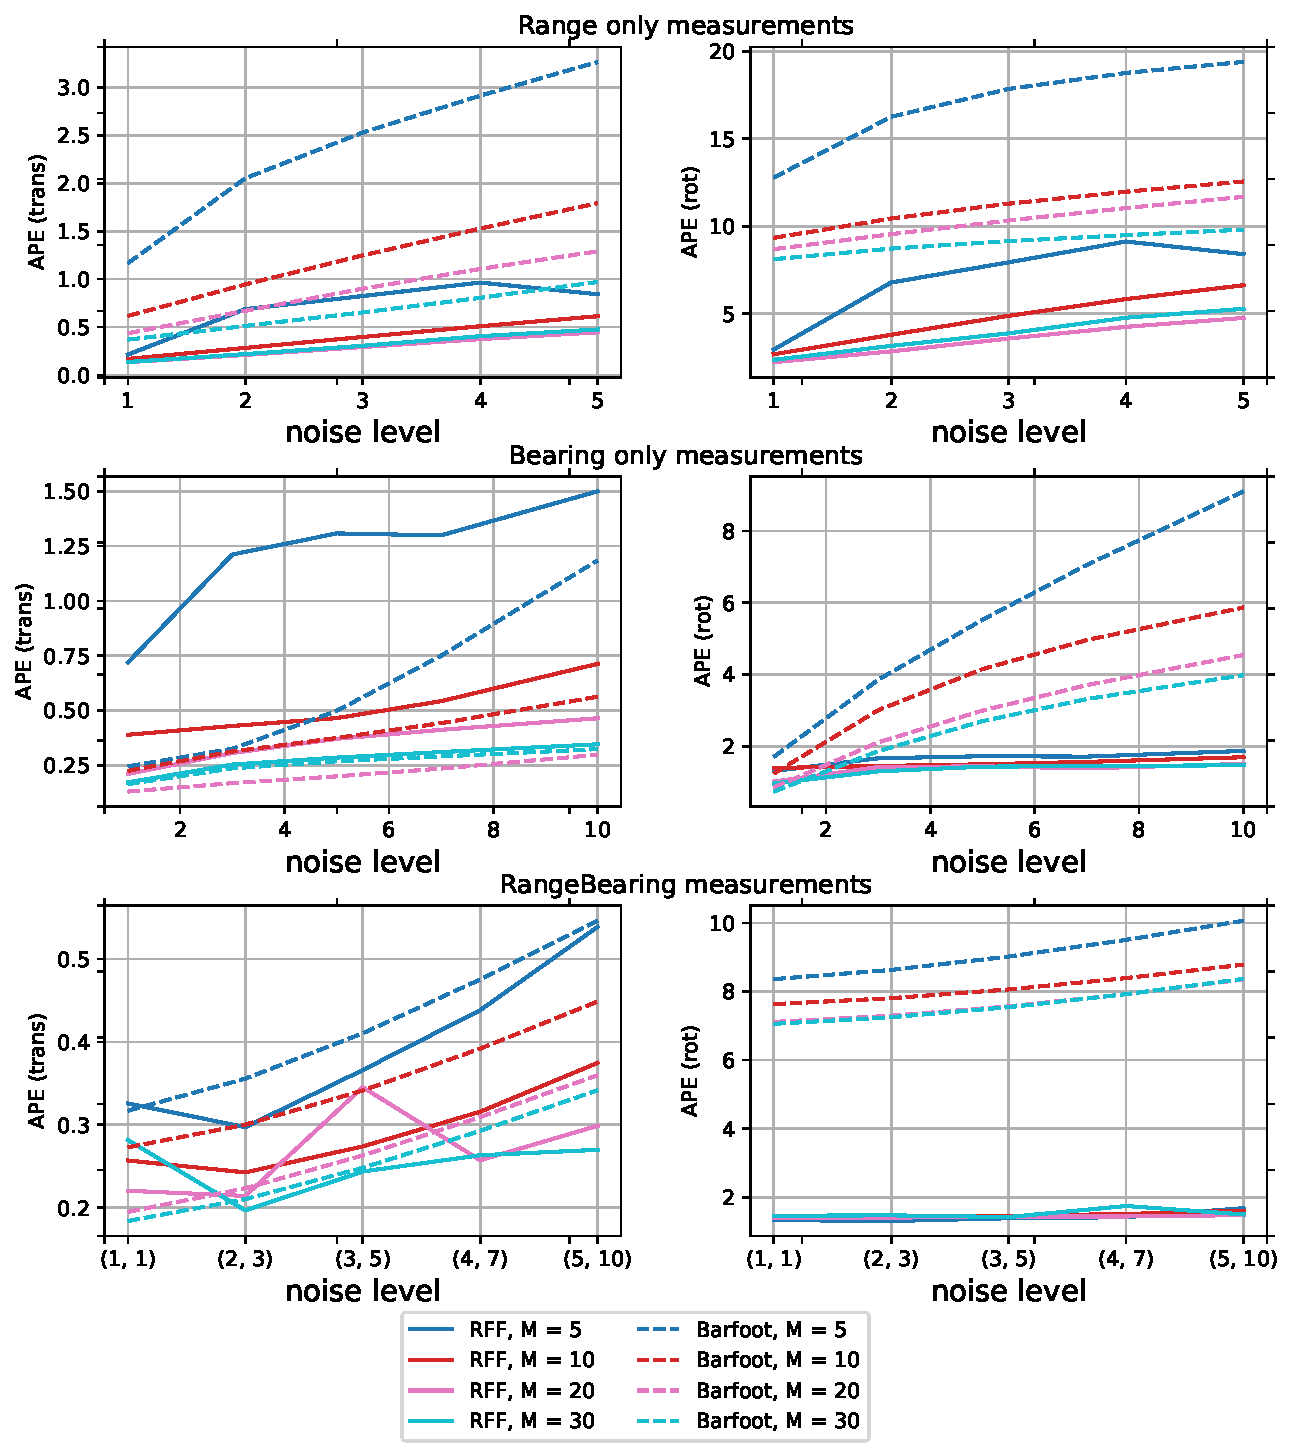
\includegraphics[width=0.8\textwidth]{figures/slam/synthetic_noise_distr.pdf}
    \caption{Average APE errors for synthetic trajectories at different noise levels
    and number of landmarks}
    \label{fig:synthetic_noise_distr}
\end{figure}

\begin{table}[]
    \centering
    \caption{Relative Errors for synthetic trajectories}
    \label{tab:rand_2d_errors}
    \begin{tabular}{cc|c c c}
     & & Pos. & Rot. & Landmarks \\
     \toprule
     RangeBearing & RFF & 0.022 & \textbf{0.154} & 6e-4 \\
     & LTV SDE & 0.025 & 5.602 & 0.110 \\
     \hline
     Range & RFF & \textbf{0.016} & \textbf{0.320} & 1e-6 \\
     & LTV SDE & 0.025 & 5.580 & 0.003 \\
     \hline
     Bearing & RFF & 0.035 & \textbf{0.152} & 8e-6 \\
     & LTV SDE & \textbf{0.025} & 1.200 & 0.016 \\
     \bottomrule
    \end{tabular}
\end{table}


\subsubsection{Autonomous Lawn-Mower}
In this experiment we evaluate our approach on a Plaza data set
collected from an autonomous
lawn-mower~\cite{djugash2010geolocation}.
The data set contains range measurements recorded using
time-of-flight and odometry measurements.
Odometry measurements come more frequently than range measurements.
The ground truth data was collected from GPS measurements
and according to \cite{djugash2010geolocation} its accuracy
is $2$cm.

The resulting trajectory is given in
Figure~\ref{fig:autnomous_lawn_mower}.
In this experiment we did batch updates, i.e.
we updated the trajectory after each new $5$ range measurements.
The motion model based prior was used as we have odometry
measurements.
We can see slight oscillations of the estimated trajectory.
They can be explained by the nature of the Fourier features.
However, the errors are comparable as can be seen from Table~\ref{tab:real_benchmarks_errors}.
The estimated trajectories are depicted in Figure~\ref{fig:autnomous_lawn_mower}.

\begin{figure}[h]
    \centering
    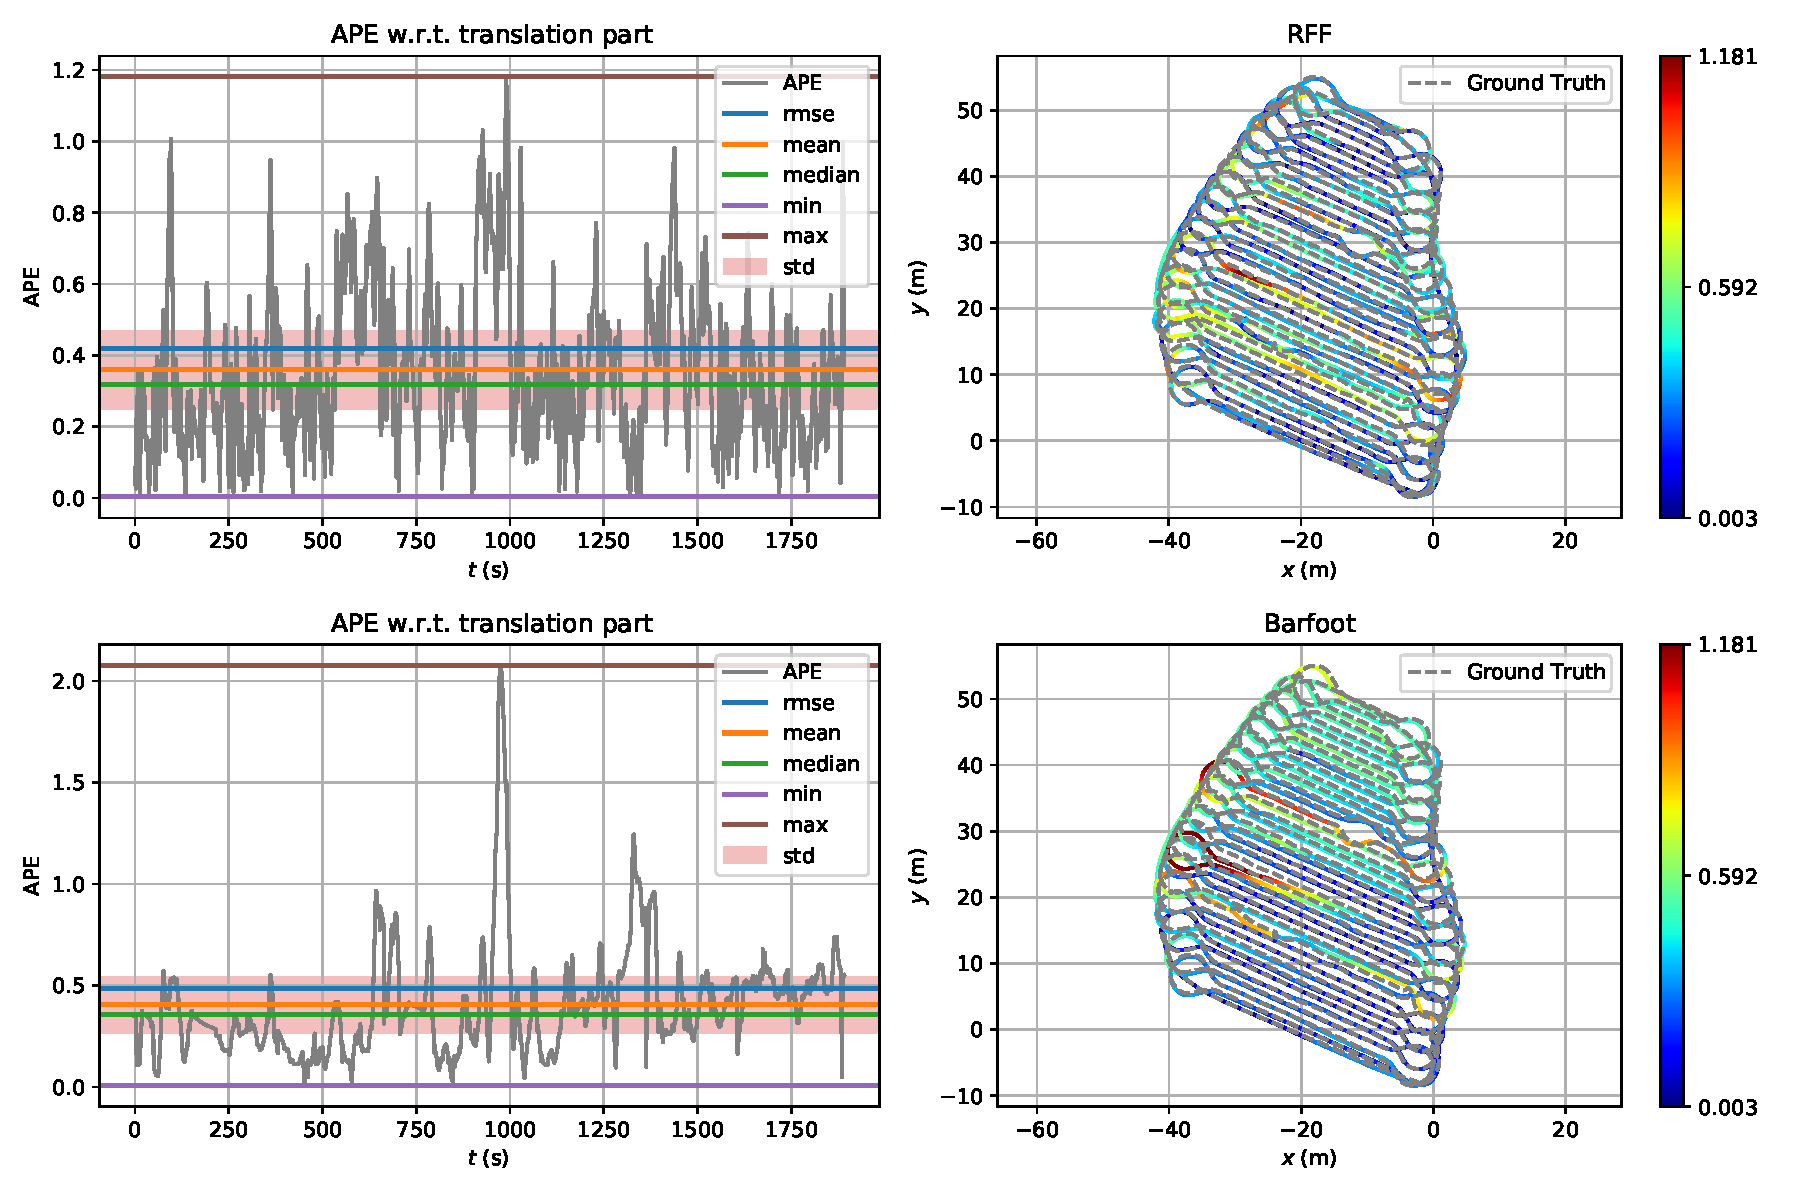
\includegraphics[width=0.8\textwidth]{figures/slam/plaza_ape.pdf}
    \caption{Distribution of APE errors along the trajecotry for Autonomous Lawn-Mower benchmark}
    \label{fig:autnomous_lawn_mower}
\end{figure}

\subsubsection{KITTI-projected dataset}

To evaluate our approach, we proceed with the world-famous dataset KITTI odometry\cite{kitti}.
We chose the dataset part that contains stereo sequences -- a sequence of stereo images taken while moving along a
specific trajectory.
The dataset includes stereo images, ground truth trajectory and camera information.
For our approach, we need a dataset in 2D with observations and bearing.
To extract observations in the form \eqref{eq:observation_function} we do visual SLAM from ORB-SLAM2 \cite{mur2017orb}.
For each keypoint we find its coordinates in the local frame\cite{multiview}.
Therefore, we can calculate bearing observations for each keypoint.
Thus, the keypoints in this case play the role of landmarks and we have bearing measurements.
The pipeline to project KITTI into a 2D dataset is following:

\begin{itemize}
\item Input: KITTI-odometry dataset (e.g. sequence 08);
\item Run ORB-SLAM2 to get observations (keypoints, timestamps);
\item Correct camera pose and keypoints by a transformation term that aligns with the vertical axis to make them independent of their original camera pose
\begin{equation}  \label{eq:corr}
R_t \cdot R_{correction} = \mathrm{Exp}([0,0,\alpha]^{\top});
\end{equation}
\item Calculate weights for each observations based on how much time this point was observed/visited;
\item Filter observations;
\item Do orthonormal projection for each observation;
\item Calculate bearing.
\end{itemize}

The number of landmarks (keypoints) is $80771$.
With such a big number of landmarks, the experiments are very slow, so we reduced the number of landmarks to $3975$.
We selected the landmarks randomly with probabilities proportional to their weights, but for each keyframe
we left not less than $10$ landmarks.
Also, to speed up the calculations we split the trajectory
into $10$ consecutive slices, do estimation on each slice
independently and then average the estimation errors.

The extracted data we then use in our approach to estimate the trajectory.
To check our assumption that kernels with dense precision
matrices should work better in case of noisy observations,
we also generated a noisy version of the KITTI-projected
dataset.
To do so, we added Gaussian noise with standard deviation $\sigma$.

The results are given in Table~\ref{tab:real_benchmarks_errors}.
We can see that without additional noise the results are comparable (with RFF based approach being slightly better).
When we increase the amount of noise, absolute errors of our approach remains the same
while errors for LTV SDE increase.

\begin{table}[ht]
    \centering
    \caption{Real-world benchmark errors.}
    \label{tab:real_benchmarks_errors}
    \begin{tabular}{c|c|c|c|c}
    \multicolumn{5}{l}{}\\[-0.5em]
    \multicolumn{5}{c}{Autonomous Lawn-Mower} \\
    \multicolumn{5}{l}{}\\[-0.7em]
    \toprule
    & APE (trans) & APE (rot) & RPE (trans) & RPE (rot) \\
    \hline
    LTV SDE & $0.48$ & $1.44$ & $0.021$ & $0.10$ \\
    RFF & $0.42$ & $2.25$ & $0.026$ & $0.54$ \\
    \bottomrule

    \multicolumn{5}{l}{}\\[-0.5em]
    \multicolumn{5}{c}{KITTI-projected} \\
    \multicolumn{5}{l}{}\\[-0.7em]
    \toprule
    LTV SDE & $5.130$ & $1.059$ & $0.068$ & $0.113$ \\
    RFF & $5.070$ & $0.489$ & $0.040$ & $0.048$ \\
    \bottomrule

    \multicolumn{5}{l}{}\\[-0.5em]
    \multicolumn{5}{c}{KITTI-projected + noise, $\sigma=1^\circ$} \\
    \multicolumn{5}{l}{}\\[-0.7em]
    \toprule
    LTV SDE & $5.126$ & $1.086$ & $0.068$ & $0.133$ \\
    RFF & $5.070$ & $0.544$ & $0.0454$ & $0.052$\\
    \bottomrule

    \multicolumn{5}{l}{}\\[-0.5em]
    \multicolumn{5}{c}{KITTI-projected + noise, $\sigma=3^\circ$} \\
    \multicolumn{5}{l}{}\\[-0.7em]
    \toprule
    LTV SDE & $5.491$ & $3.136$ & $0.139$ & $0.259$ \\
    RFF & $5.075$ & $1.027$ & $0.073$ & $0.115$ \\
    \bottomrule

    \multicolumn{5}{l}{}\\[-0.5em]
    \multicolumn{5}{c}{KITTI-projected + noise, $\sigma=5^\circ$} \\
    \multicolumn{5}{l}{}\\[-0.7em]
    \toprule
    LTV SDE & $12.915$ & $5.114$ & $0.242$ & $0.358$\\
    RFF & $5.077$ & $1.304$ & $0.084$ & $0.119$ \\
    \bottomrule
    \end{tabular}
\end{table}

